\chapter{Geometrische Beziehungen zwischen Punktekorrespondenzen}
\label{sec:HFE}

Das Ziel dieser Masterarbeit ist es Punkte im dreidimensionalen Raum aus einer Stereoskopischen Aufnahme zweier Kameras zu rekonstruieren. Bisher wurde die Bildaufnahme einer einzigen Kamera betrachtet. Jedoch kann eine Kamera allein nicht räumlich sehen. Um dreidimensionale Szenen aus Bilder zu rekonstruieren, müssen mindestens zwei Aufnahmen der gleichen Szene aus unterschiedlichen Blickwinkeln aufgenommen werden. Innerhalb dieser Aufnahmen müssen Punktekorrespondenzen gesucht werden. Korrespondierende Punkte zeichnen sich dadurch aus, dass sie die Abbildungen desselben Ursprungspunktes im Raum sind. Für diese Punkte muss dann eine gemeinsame Abbildungsvorschrift aufgestellt werden. Mit diesen Abbildungsvorschriften ist es möglich eine Beziehung zwischen zwei projizierten Bildpunkten 
herzuleiten. Die Abbildungsvorschrift wird in einer $3 \times 3$-Matrix $H$ ausgedrückt, welche die Transformationsmatrizen, sowie die Kameramatrizen zusammenfasst. Die $3 \times 3$-Matrix, kann aus gegebenen Punktekorrespondenzen abgeleitet werden. Aus $H$ können Rückschlüssen auf die Kameraparameter der beiden Kameras gezogen werden.  \\


%
%Über die Abbildungsvorschrift können dann Schlüsse auf die Kameraparameter der beiden Kameras gezogen werden. Im ersten Schritt wird eine Abbildungsvorschrift für die Korrespondenzanalyse von Punkten auf einer Ebene aufgestellt. Im zweiten Schritt wird diese Abbildungsvorschrift für die Korrespondenz zwischen willkürlichen Punkten im Raum entsprechend erweitert. \\

Es seien \ensuremath{m_{\tau} =(m_{\tau,1},m_{\tau,2},m_{\tau,3})^T} die homogenen Koordinaten eines Punktes auf der Bildebene$(I,\tau)$ und \ensuremath{m'_{\tau'} = (m'_{\tau',1},m'_{\tau',2},m'_{\tau',3})^T} der dazu Korrespondierende Punkt der projektiv transformierten Bildebene $(I',\tau')$. Gesucht wird eine Abbildungsvorschift welche als Matrix H ausgedrückt wird:

\begin{gather}
	m'_{\tau'} = Hm_{\tau}\\
	Hm_{\tau} = \begin{bmatrix}
		{h_1}^T \cdot m_{\tau,1}\\{h_2}^T \cdot m_{\tau,2}\\{h_3}^T \cdot m_{\tau,3}
	\end{bmatrix} \\
	\leadsto 
	m'_{\tau'}= Hm_{\tau}= \begin{bmatrix}
		h_{11}m_{\tau,1}+h_{12}m_{\tau,2}+h_{13}m_{\tau,3}\\
		h_{21}m_{\tau,1}+h_{22}m_{\tau,2}+h_{23}m_{\tau,3}\\
		h_{31}m_{\tau,1}+h_{32}m_{\tau,2}+h_{33}m_{\tau,3}
	\end{bmatrix}\\
	\leadsto 
	H=\begin{bmatrix}
		h_{11}&h_{12}&h_{13}\\
		h_{21}&h_{22}&h_{23}\\
		h_{31}&h_{32}&h_{33}
	\end{bmatrix}
\end{gather}

%Im folgenden werden zunächst zwei Fälle für die Herleitung von Abbildungsvorschriften unterschieden.

In den ersten beiden Abschnitten werden zwei Herleitungen der gesuchten Abbildungsvorschriften, in zwei unterschiedlichen Fällen, anhand von bekannten Transformationsmatrizen und Kameramatrizen aufgezeigt. 
Im ersten Fall wird davon ausgegangen, dass die 3D-Punkte im Raum auf einer Ebene liegen und auf die Bildebenen von zwei zueinander verschobenen und rotierten Kameras abgebildet werden. Im zweiten Fall werden die Punkte eines komplexeren 3D-Objektes auf die beiden Bildebenen abgebildet. Im letzten Abschnitt werden dann die Herleitungen der entstehenden Matrizen beider Fälle für den Fall von unbekannten Kameraparameter aufgezeigt. 


\section{Korrespondenzanalyse für Punkte auf einer Ebene (Homographie)}

Eine Abbildungsvorschrift kann in bestimmten Fällen eindeutig bestimmt werden. In diesen Fällen nennt man die Abbildung zwischen beiden zweidimensionalen Bildern Homographie\cite{HZ,Elements,Roser}. In diesem Kapitel wird der beispielhafte Fall behandelt, dass Punkte auf der $x,y$-Ebene im Weltkoordinatensystem auf zwei unterschiedlichen Kameras $C$ und $C'$ abgebildet wird. Dies ist in Abbildung dargestellt.

\begin{minipage}{\linewidth}
	\centering
	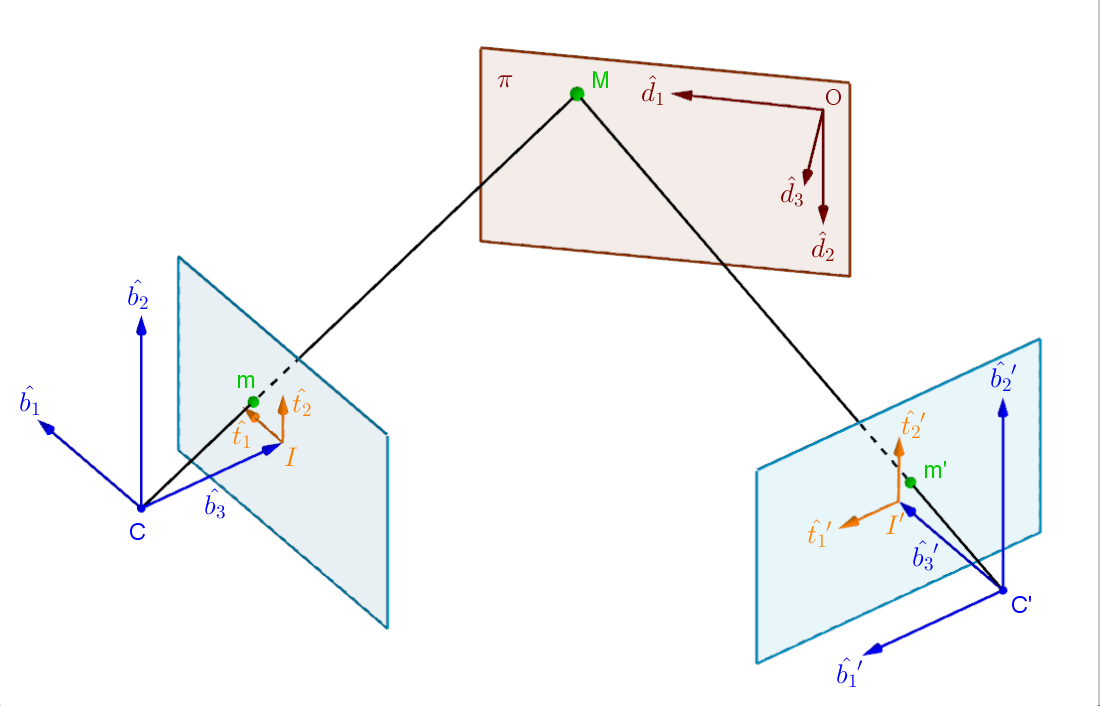
\includegraphics[width=0.8\linewidth]{images/HomographieDP_beschriftet.png}
	\captionof{figure}{In der Abblidung sind die beiden Kameras $C$ und $C'$ mit ihren Bildebenen $I$ und $I'$ zu sehen. Ein Objektpunkt $M_\delta$ bezüglich eines Weltkoordinatensystems $(O,\delta)$ befindet sich auf der Ebene $\pi$, welche durch die Achsen $\hat{d_1}$ und $\hat{d_2}$ aufgespannt wird. $M_\delta$ wird auf $I$ und $I'$ projiziert. Es entstehen die Bildpunkte $\gamma m_\tau$ und $\gamma' m'_\tau$.}  
	\label{fig:Homographie}
\end{minipage}\\

Um die Abbildungsvorschrift herzuleiten beginnen wir bei dem Bildpunkt \ensuremath{m_{\tau} = (m_{\tau,1},m_{\tau,2},m'_{\tau,3})^T} mit $m_{\tau,3}=1$. Während in der Bildaufnahme ein Punkt $m_\beta$ durch Division mit der $m_{\beta,3}$-Komponenten eindeutig zu $m_{\tau}$ wird ist die Rückrichtung nicht eindeutig. Alle Punkte auf der Geraden von C und $m_{\tau}$, siehe Abbildung \ref{fig:gamma},werden auf denselben Bildpunkt projiziert. Die Projektion von $m_{\tau}$ auf $m_\beta$ ist demnach nicht eindeutig. Die Gerade mit allen möglichen Punkten $m_\beta$ kann als $\gamma m_{\tau}$, mit der freien Variablen $\gamma > 0$ ausgedrückt werden.  


\begin{minipage}{\linewidth}
	\centering
	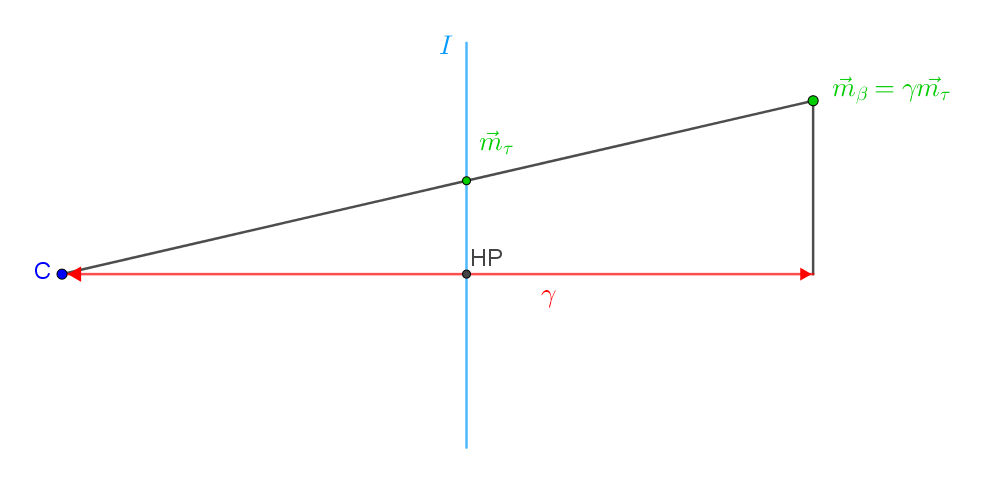
\includegraphics[width=0.8\linewidth]{images/gamma.png}
	\captionof{figure}{ }  
	\label{fig:gamma}
\end{minipage}\\
%Ein Punkt $M_\delta$ bezüglich eines Weltkoordinatensystems $(O,\delta)$ mit $\delta = (\hat{d_1},\hat{d_2},\hat{d_3},O)$, wird auf zwei Bildebenen $(I,\tau)$ und $(I',\tau')$ projiziert. 
Für zwei korrespondierende Bildpunkte $m_\tau$ und $ m'_{\tau'}$ kann für die möglichen Punkte $m_\beta$ und $m'_\beta$ die folgende Projektionsvorschrift hergeleitet werden \cite{Elements}.

\begin{gather}
	\gamma \vec{m}_\tau = P \begin{bmatrix}\vec{M}_\delta\\1\end{bmatrix} = 
	\begin{bmatrix}KR|-KR\vec{C}_\delta\end{bmatrix}\cdot \begin{bmatrix}\vec{M}\delta\\1\end{bmatrix} = KR(\vec{M}\delta - \vec{C}_\delta)\\
	\gamma' \vec{m'_{\tau'}} = P' \begin{bmatrix}\vec{M'}_\delta\\1\end{bmatrix} = 
	\begin{bmatrix}K'R'|-K'R'\vec{C'}_\delta\end{bmatrix}\cdot \begin{bmatrix}\vec{M}\delta\\1\end{bmatrix} = K'R'(\vec{M}\delta - \vec{C'}_\delta)\label{eq:Homo}
\end{gather}


%$\gamma m_\tau$ und $\gamma m'_{\tau'}$ stehen für die nicht-normierten Kamerakoordinaten mit einer willkürlichen Tiefe $\gamma$.Zur Erinnerung in Kapitel ?? wurde in Gleichung \ref{eq:21} ein 3D-Punkt $M_\delta$ auf eine Bildebene projiziert. Der entstandene Punkt $m_\tau$ hatte bei einer bekannten Tiefe $Z$ die Form $	m_\tau = \begin{pmatrix}
%\zeta X\\ \zeta Y\\Z
%\end{pmatrix} $, man spricht hier von einer nicht-normierten Bildebenenkoordinate. Durch normierung wird aus $m_\tau$ eine zweidimensionale Bildebenkoordinate mit $m_\tau = \begin{pmatrix}
%\frac{\zeta X}{Z}\\ \frac{\zeta Y}{Z}
%\end{pmatrix}$.Für die Rücktransformation der normierten auf die nicht-normierten Bildebenkooridnaten wurde eifnach wieder mit $Z$ erweitert.\\

%Für die Herleitung der Abbildungsvorschriften, wird in beiden Fällen davon ausgegangen dass die Tiefe $Z$ willkürlich ist und so wird der nicht normierte Bildebenpunkt $m_\tau$ mit einer undefinierten Tiefe $\gamma$ eweitert\cite{Elements}. So das gilt:

%\begin{gather}
%	\begin{pmatrix}
%		\frac{\zeta X}{\gamma}\\ \frac{\zeta Y}{\gamma}
%	\end{pmatrix}
% \leadsto 
% \begin{pmatrix}
%		\zeta X\\ \zeta Y\\\gamma
%	\end{pmatrix}
%\end{gather}\\


%Für den F gilt der ein bestimmter Szenenaufbau. Es existiert eine Ebene $\pi$ im Raum, auf welcher sich ein Objektpunkt $M_\delta$ bezüglich eines Weltkoordinatesystems $(O,\delta)$ befindet. Die Achsen $\hat{d_1}$ und $\hat{d_2}$ von $O$ spannen die Ebene $\pi$ auf. Der Punkt $M_\delta$ wird nun mit den Projektionsmatrizen $P = [KR|-KR\vec{C}_\delta]$ und $P'=	[K'R'|-K'R'\vec{C}_\delta]$ in einen Punkt bezüglich der Bildebenen $(I,\tau)$ mit $\tau = (\hat{t_1}, \hat{t_2},I)$ und $(I',\tau')$ mit $\tau' = (\hat{t_1}', \hat{t_2}',I')$ projiziert. Es entstehen zunächst die nicht-normierten Bildebenkoordinaten $\gamma m_\tau$ und $\gamma m'_{\tau'}$.  Da der Ursprung des Weltkoordinatensystem $(O,\delta)$ auf der Ebene $\pi$ liegt, gilt für den Punt $M_\delta$ auf $\pi$ $M_\delta = \begin{pmatrix}
%x_{\hat{d_1}}\\
%y_{\hat{d_2}}\\
%0
%\end{pmatrix}$. Abbildung \ref{fig:Homographie} veranschaulicht den eben beschrieben Aufbau noch einmal grafisch.

%(GRAFIK NOCH AKTUALISIEREN)\\
%\begin{minipage}{\linewidth}
%	\centering
%	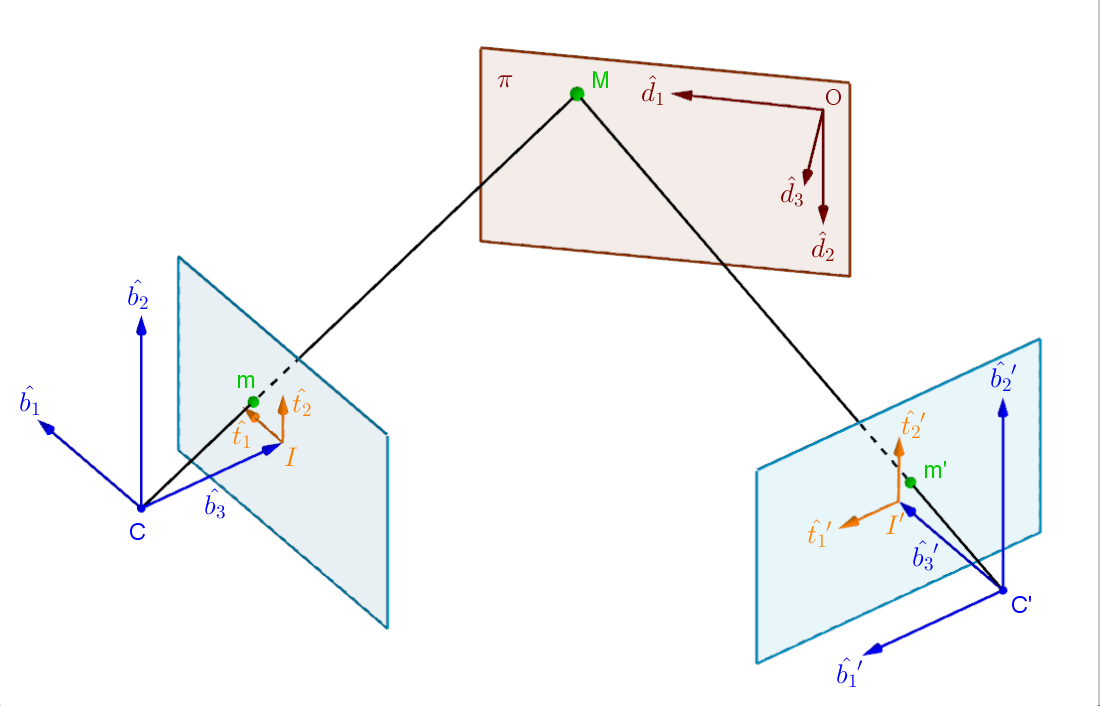
\includegraphics[width=0.8\linewidth]{images/HomographieDP_beschriftet.png}
%	\captionof{figure}{In der Abblidung sind die beiden Kameras $C$ und $C'$ mit ihren Bildebenen $I$ und $I'$ zu sehen. Ein Objektpunkt $M_\delta$ bezüglich eines Weltkoordinatensystems $(O,\delta)$ befindet sich auf der Ebene $\pi$, welche durch die Achsen $\hat{d_1}$ und $\hat{d_2}$ aufgespannt wird. $M_\delta$ wird auf $I$ und $I'$ projiziert. Es entstehen die Bildpunkte $\gamma m_\tau$ und $\gamma' m'_\tau$.}  
%	\label{fig:Homographie}
%\end{minipage}\\

Mit einem Ursprungspunkt $M_\delta=(x_\delta,y_\delta,0)^T$ auf der x,y Ebene im Weltkoordinatensystem und einer unbekannten Projektionsmatrix P mit

\begin{gather}
	P=
	\begin{bmatrix}
		p_{11}&p_{21}&p_{31}&p_{41}\\
		p_{12}&p_{22}&p_{32}&p_{42}\\
		p_{13}&p_{23}&p_{33}&p_{43}
	\end{bmatrix}=	\begin{bmatrix}
		p_1&p_2&p_3&p_4
	\end{bmatrix}
\end{gather} 

kann die folgende Gleichung aufgestellt werden \cite{Elements}


\begin{gather}
	\gamma m_\tau = P \cdot 
	\begin{bmatrix}
		M_\delta\\1
	\end{bmatrix} = 
	\begin{bmatrix}
		p_1&p_2&p_3&p_4
	\end{bmatrix} \cdot
	\begin{bmatrix}
		x_\delta\\y_\delta\\0\\1
	\end{bmatrix}=
	\begin{bmatrix}
		p_1&p_2&p_4
	\end{bmatrix} \cdot
	\begin{bmatrix}
		x_\delta\\y_\delta\\1
	\end{bmatrix}=
	G \vec{m}_\delta\\
	\gamma' m'_{\tau'} = P \cdot 
	\begin{bmatrix}
		M_\delta\\1
	\end{bmatrix} = 
	\begin{bmatrix}
		p'_1&p'_2&p'_3&p'_4
	\end{bmatrix} \cdot
	\begin{bmatrix}
		x_\delta\\y_\delta\\0\\1
	\end{bmatrix}=
	\begin{bmatrix}
		p'_1&p'_2&p'_4
	\end{bmatrix} \cdot
	\begin{bmatrix}
		x_\delta\\y_\delta\\1
	\end{bmatrix}=
	G' \vec{m}_{\delta}. 
\end{gather}\\


Aus $\gamma m_\tau = G\cdot m_\delta$ und $\gamma' m'_{\tau'} = G'\cdot m_{\delta}$ kann dann folgendes abgeleitet werden\cite{Elements}.

\begin{gather}
	\gamma' m'_{\tau'} = G' G^{-1} \gamma m_\tau \label{eq:gammaTau}
\end{gather}

Mit $\lambda= \frac{\gamma'}{\gamma}$, kann Gleichung \ref{eq:gammaTau} dann wieder umformuliert werden und in die Bedienungsgleichung der Homographie mit $H=G' G^{-1}$ umgeformt werden:

\begin{gather}
	\lambda m'_{\tau'} = H m_\tau\label{eq:H}
	%\leadsto m'_{\tau'} = H m_\tau, 
\end{gather} 


Die entstandene Homographie $H$ ist somit eine Abbildungsvorschrift welche zwei korrespondierende Punkte in Verbindung setzt \cite{Elements}. %$\lambda= \frac{\gamma'}{\gamma}$ ist ein Mass für den Relativen unterschied der Distanz zwischen beiden Kameras zum Bildpunkt.
Diese Homographiebedingung stellt ein Gleichungssystem mit 9 unbekannten, welche in Kapitel 3.2 gelöst wird\cite{HZ}.

% (WO ist die verbindung zur rektifizierung, wie stell ich verbindung von H zur projektionsmatrix her?) 


% %Ein Punkt auf der normierten Bildebene m_{n,\tau}=(m_{n,\tau x},m_{n,\tau y},1, I) lässt sich somit eindeutig zurücktransformieren indem die Gerade $\g=vec(C)+t\vec(Cm)
% 
% Ein Punkt auf der normierten Bildebene $m_{n,\tau}=(m_{n,\tau x},m_{n,\tau y},1, I)$ lässt sich somit eindeutig auf die Bildebene erweitern mit 
% 
% \begin{gather}
% 	m_{\tau}=(m_{\tau x},m_{\tau y},m_{\tau z}, I) = M_{\delta z}(m_{n,\tau x},m_{n,\tau y},1, I)=M_{\delta z}m_{n,\tau}
% \end{gather}\\
% 
% Für 2 korrespondierende Punkte $m_{\tau}$ und $m'_{\tau}$ auf 2 unterschiedlichen Bildebenen gilt der folgende Zusammenhang
% 
% 
% \begin{gather}
% 	m_{\tau}=M_{\delta z}m_{n,\tau} = M_{\delta} \cdot P \\
% 	m'_{\tau}=M_{\delta z}m'_{n,\tau} = M_{\delta} \cdot P'
% \end{gather}\\
% 
% Die Projektionsmatirx $P$ beschriebt in diesem Fall nur die Abbildung auf die Bildebene und wird durch $P=K_0R$ mit der Kameramatrix $K_0$ und der Transformationsmatrix $R$ aus Kapitel 2 zusammen. Durch das Anwenden der inversen von $P$ und $P'$ von rechts auf die gleichung, werden diese zu
% 
% 
% \begin{gather}
% 	m_{\tau}\cdot P^{-1}=M_{\delta z}m_{n,\tau}P^{-1} = M_{\delta} \\
% 	m'_{\tau}P'^{-1}=M_{\delta z}m'_{n,\tau}P'^{-1} = M_{\delta}.
% \end{gather}\\
% 
% Auf der rechten Seite der Gleichung steht schließlich derselbe Ursprungspunkt, sodass wir beide gleichung zusammenfassen können. 
% 
% \begin{gather}
% 	m_{\tau}\cdot P^{-1} = m'_{\tau}P'^{-1} \\
% 	m_{n,\tau}P^{-1}=m'_{n,\tau}P'^{-1}
% \end{gather}\\
% 
% Multiplizieren wir nun P von rechts auf die Gleichung erhalten wir 
% \begin{gather}
% 	m_{n,\tau}=m'_{n,\tau}P'^{-1}P=m'_{n,\tau}H
% \end{gather}\\
% 
%die sogenannte Homographiematirx $H=P'^{-1}P$. Diese Matrix beschreibt die direkte, eindeutige Abbildung von einem Bildpunkt auf der 2 dimensionalen Bildebene I' auf den Bildpunkt auf der Bildebene I. Mittels der inversen $Hi$ kann diese Abbildung auch rückwerts gemacht werden. 
% \\
% Mann könnte das gleichungssystem hier ausformulieren um auf die bestimmung der Kameraparameter einzugehn, wenn du willst (denke das hilft hier zwar nicht aber schaden tut warhscheinlich auch nicht so sehr)
% 


\section{Korrespondenzanalyse für willkürliche Punkte im Raum (Epipolare Geometrie)}

Für Bilder von dreidimensionalen Objekten, bei denen die Punkte auf verschiedenen Ebenen liegen können, kann keine Homographiebedingung hergestellt werden um die Kameraparameter zu bestimmen. Jedoch kann auf geometrische Bedingungen zurückgegriffen werden mit denen die Abbildungsvorschrift zwischen den Bildern ausgenutzt werden um die Kameraparameter beider Kameras zu bestimmen. Ein Ursprungspunkt $M_\delta$ wird wieder mit zwei Kameras $C$ und $C'$ aufgenommen. In Abbildung \ref{fig:Epipolargeometry} ist das stereoskopische System dargestellt . 


\begin{minipage}{\linewidth}
	\centering
	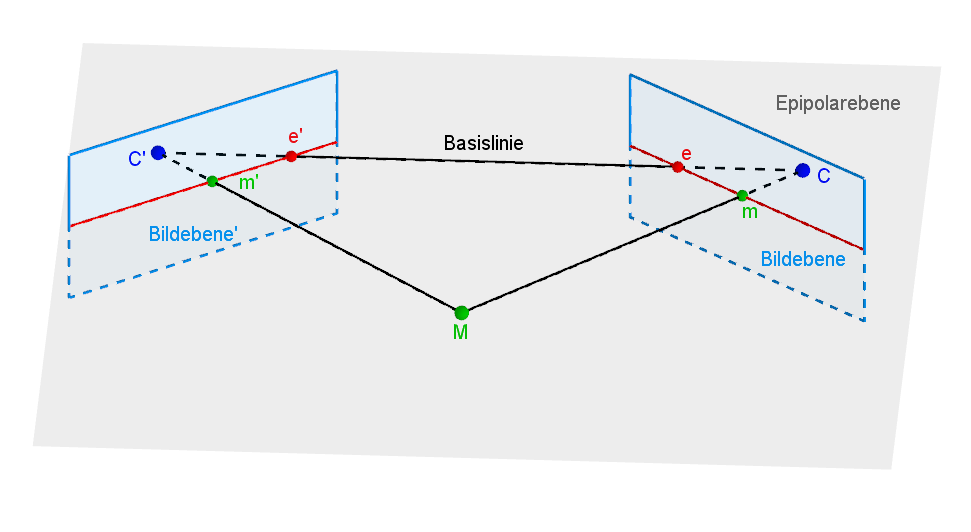
\includegraphics[width=.8\linewidth]{images/EpipolarGeoemtrieGrafik.png}
	\captionof{figure}{$C$ und $C'$ sind die Projektionszentren zweier Kameras. Beide Kameras besitzen jeweils eine Bildebene. Die Basislinien verbindet die Projektionszentren der Kameras. Die Punkte an welchen die Basislinie die Bildebenen schneidet, werden als Epipole $e$ und $e'$ bezeichnet. Durch einen Epipol verlaufen alle Epipolarlinien des Bildes. $M$ ist der Objektpunkt im 3D-Raum und $m_1$ und $m_2$ sind die jeweiligen Abbildungen dieses Punktes auf den Bildebenen. Die Verbindungsvektoren zwischen $C, C'$ und $M$ bilden die sogenannte Epipolarebene\cite{Elements,HZ,ZZGXr}.}  
	\label{fig:Epipolargeometry}
\end{minipage}\\ \\

Es werden hier einige Definitionen eingeführt und die Berechnung geometrisch Motiviert um die danach folgende mathematische Herleitung genauer zu verstehen. Die Vektoren $\overline{CM} = (\vec{M}_\delta - \vec{C}_\delta),\, \overline{C'M} = (\vec{M}_\delta - \vec{C'}_\delta)$ und $\overline{CC'} = (\vec{C'}_\delta - \vec{C}_\delta)$ definieren die Epipolarebene, die durch das schwarze Dreieck in Abbildung \ref{fig:Epipolargeometry} gekennzeichnet ist. Der Schnittpunkt der Gerade zwischen $C$ und $C'$ mit der jeweiligen Bildebene $I$ und $I'$ werden als Epipole $e$ und $e'$ bezeichnet. Die Schnittgerade der Epipolarebene mit $I$ und $I'$ bilden die sogenannten Epipolarlinien $l$ und $l'$\cite{HZ,Zhang2014,ZZPaper,Elements}.\\

Ein Bildpunkt $m_i$ auf der Bildebene $I$ wird zuerst auf die Gerade, die durch $m_i$ und $C$ geht abgebildet. Die Gerade stellt alle möglichen Ursprungspunkte zu $m_i$ da. Dies ist durch die drei möglichen Punkte $M1$,$M2$,$M3$ in Figur \ref{fig:Epipolarconstraint} dargestellt. Jeder dieser Punkte wird nun wiederum auf I' projiziert. Die so entstandenen Punkte liegen alle auf der Epipolarlinie $l'$\cite{HZ}. 

\begin{minipage}{\linewidth}
	\centering
	\includegraphics[width=.8\linewidth]{images/EpipolarLinien.png}
	\captionof{figure}{Die Objektpunkte $M_1, M_2$ und $M_3$ werden in $I'$ als $m'_1, m'_2$ und $m'_3$ abgebildet, während sie in $I$ immer den selben Bildpunkt $m_1$ ergeben.}  
	\label{fig:Epipolarconstraint}
\end{minipage}\\ \\



Die hier gezeigte Abbildung von $mi$ auf $l'$ wird nun genauer betrachtet. Es werden wieder die Gleichungen für $m_\tau$ und $m'_\tau$, wie in Gleichung \ref{eq:Homo}, aufgestellt    

\begin{gather}
	\gamma \vec{m}_\tau = P \begin{bmatrix}\vec{M}_\delta\\1\end{bmatrix} = 
	\begin{bmatrix}KR|-KR\vec{C}_\delta\end{bmatrix}\cdot \begin{bmatrix}\vec{M}\delta\\1\end{bmatrix} = KR(\vec{M}\delta - \vec{C}_\delta) \label{eq:Ep1} \\
	\gamma' \vec{m'_{\tau'}} = P' \begin{bmatrix}\vec{M'}_\delta\\1\end{bmatrix} = 
	\begin{bmatrix}K'R'|-K'R'\vec{C'}_\delta\end{bmatrix}\cdot \begin{bmatrix}\vec{M}\delta\\1\end{bmatrix} = K'R'(\vec{M}\delta - \vec{C'}_\delta)\label{eq:Ep2}
\end{gather}


Gleichungen \ref{eq:Ep1} und \ref{eq:Ep2} werden nach $(\vec{M}-\vec{C}_\delta)$ und $(\vec{M}-\vec{C'}_\delta)$ aufgelöst.

\begin{gather}
	\gamma R^TK^{-1}\vec{m}_\tau = (\vec{M}-\vec{C}_\delta)\label{eq:Ep3}\\
	\gamma' R'^TK'^{-1}\vec{m'}_{\tau'} = (\vec{M}-\vec{C'}_\delta)\label{eq:Ep4}
\end{gather}


Wie in Abbildung \ref{fig:Epipolargeometry} gezeigt bilden Vektoren $(\vec{M}_\delta - \vec{C}_\delta),\, (\vec{M}_\delta - \vec{C'}_\delta)$ und $(\vec{C'}_\delta - \vec{C}_\delta)$ ein Dreieck. Für dieses Dreieck kann die folgende Gleichung aufgestellt werden. 

\begin{gather}
	(\vec{C'}_\delta - \vec{C}_\delta) = (\vec{M}_\delta - \vec{C}_\delta) - (\vec{M}_\delta - \vec{C'}_\delta)
\end{gather}

$(\vec{M}-\vec{C}_\delta)$ und $(\vec{M} - \vec{C'}_\delta)$ können durch die Ausdrücke in den Gleichungen \ref{eq:Ep3} und \ref{eq:Ep4} ersetzt werden um folgende Gleichung zu erhalten

\begin{gather}
	(\vec{C'}_\delta - \vec{C}_\delta) = \gamma' R^TK^{-1}\vec{m}_\tau - \gamma R'^TK'^{-1}\vec{m'}_{\tau'}. \label{eq:Ep5}
\end{gather}

Durch Vektoridentitäten können $\gamma$ und $\gamma'$ elimiert werden und folgende Bedingung  aus Gleichung \ref{eq:Ep5} hergeleitet werden \cite{Elements} 

\begin{gather}
	0=\vec{m'_\tau}^T(K'^-1)^TR' \left[ \vec{C'_\delta}-\vec{C_\delta}\right]_\times R^TK^{-1}\vec{m_\tau}=\vec{m'_\tau}F\vec{m_\tau}\label{eq:Ep6}
	%0=\vec{m'_\tau}F\vec{m_\tau}
\end{gather}
mit  

\begin{gather}
	\left[ \vec{C'_\delta}-\vec{C_\delta}\right]_\times=
	\begin{bmatrix}0&-(C'_{z\delta}-C_{z\delta})&C'_{y\delta}-C_{y\delta}\\
		C'_{z\delta}-C_{z\delta}&0&-(C'_{x\delta}-C_{x\delta})\\
		-(C'_{y\delta}-C_{y\delta})&C'_{x \delta}-C_{x\delta}&0\\
	\end{bmatrix}.
	%0=\vec{m'_\tau}F\vec{m_\tau}
\end{gather}

In Gleichung \ref{eq:Ep6} wurde die Bedingungsgleichung für die sogenannte Fundamentalmatrix $F$ definiert. 

Sind die Kameraparameter und dadurch die Kameramatrix $K$ bekannt, so wird die essentielle Matrix $E=R' \left[ \vec{C'_\delta}-\vec{C_\delta}\right]_x R^T$ definiert. Gleichung \ref{eq:Ep6} kann zu einer Bedingung für die $E$ umgeformt werden.
\begin{gather}
	0=\vec{m'_\tau}^TK'^{-T}EK^{-1}\vec{m_\tau}\label{eq:Ep7}
\end{gather}

Gleichung \ref{eq:Ep6} oder \ref{eq:Ep7} kann verwendet werden um die Fundamentalmatrix oder essentielle Matrix aus bekannten Korrespondierenden Punkten zu bestimmen. Für die essentielle muss vorher aber noch die Koordinaten der Form

\begin{gather}
	\vec{\hat{m}}'_\tau = \vec{m'_\tau}^TK'^{-T}\\
	\vec{\hat{m}}_\tau = K^{-1}\vec{m_\tau}\label{eq:equ8}
\end{gather}

umgerechnet werden\cite{HZ}.  Der verwendete Algorithmus zur Bestimmung wird in Kapitel 3.3 näher beschrieben.\\





%Aus der Bedingung in Gleichung \ref{eq:Ep6} wird die Fundamentalmatrix definiert.



%Matrizen $F$ und $E$ ausgelesen werden. Bei $E$ handelt es sich um einen Kalibrierten Fall, dass bedeutet dass sowohl $K$ als auch $K'$ bekannt sind und die normalisierten Bildkoordinaten $\vec{\hat{m}}$ und $\vec{\hat{m}}'$  durch multiplikation mit $K$ und $K'$ entstehen. $E$ selbst fässt die Schiefsymmetrische Matrix $[\vec{C'}_\delta - \vec{C}_\delta]_\times$ und die beiden Transformationsmatrizen $R$ und $R'$ zusammen. 

%\begin{gather}
% 	\vec{m'}_{\tau'}^T K'^{-T}EK^{-1}\vec{m}_\tau = 0\\
% 	\vec{\hat{m}}_\tau^T E \vec{\hat{m}}'_{\tau'} = 0
% \end{gather}

% Matrix $E$ wird zu $F$, wenn es sich um einen unkalibrierten Fall handelt. Unkalibriert bedeutet, dass $K$ und $K'$ nicht bekannt sind, die Informationen zu $K$ und $K'$ in $F$ befinden. Werden $K$ und $K'$ zu $E'$ multipliziert, wird $E$ zu $F$. 

%\begin{gather}
%	\vec{m'}_{\tau'}^T K'^{-T}EK^{-1}\vec{m}_\tau = 0\\
%	\vec{m'}_{\tau'}^T F\vec{m}_\tau = 0
%\end{gather}

%$F$ und $E$, fassen die komplette Epipoloargeometrie, sprich externe und interne Parameter, sowie die geometrische Beziehung der jeweiligen Bildpunkte zu den 3-D Objektpunkten in einer 3x3-Matrix zusammen. Für $F$ und $E$ gibt es nicht nur eine Lösung. Werden $F$ oder $E$ Beispielsweise über den \textit{eight-Point-Algorithm} ermittelt, so sind die entstehenden 3x3-Matrixen und jedes vielfache von diesen gültige Lösungen für $F$ und $E$\cite{HZ,HZ8}. \textcolor{red}{Noch herausfinden ob das mit den Tiefen $\gamma$ und $\gamma'$ zusammenhängt!!}. Mit $F$ und $E$ kann wie bereits nachgeprüft werden, ob der \textit{epipolar-constraint} $m'^TFm = o$ oder $\hat{m'}^TE\hat{m} = 0$ zwischen zwei Bildpunkte gilt. 
Wenn die Fundamentalmatrix bekannt ist, können auch die Epipole $e$ und $e'$ und Epipolarlinien $l$ und $l'$ aus Eigenschaften den Fundamentalmatrix bestimmt werden \cite{HZ,Elements,HZ8,ZZGXr}. 

Um die Epipole $e$ zu bekommen, wird der rechte Kern von F zu bestimmt und für $e'$ muss der linke Kern von $F$ bestimmt werden\cite{HZ,Elements,HZ8,ZZGXr}.

\begin{gather}
	Fe = 0\\
	F^Te' = 0.
\end{gather}

Um die zu $m$ oder $m'$ korrespondierende Epipolarlinie $l'$ oder $l$ zu bestimmten kann die folgende Transformation verwendet werden\cite{HZ,Elements,HZ8,ZZGXr}

\begin{gather}
	l' = Fm\\
	l = F^Tm'.
\end{gather} 

Die Matrizen $F$ und $E$ sind mit diesen Eigenschaften wichtige Instrumente für die Bestimmung der Kameraorientierungen, wie im nächsten Abschnitt beschrieben wird und ihre Eigenschaften werden in den folgenden Kapiteln ausgenutzt um effiziente Rekonstruktionalgorithmen für die Szene zu implementieren. 


%In beiden folgenden Kapitel werden zwei Beispiele zur Findung der exterenen Kameraparameter und der Szenenrekonstruktion aufgezeigt. Beim ersten Beispiel handelt es sich um ein Minimalbeispiel mit synthetisch erzeugten reinen Daten, um die theoretische Funktionalität des Algorithmus zu beweisen. Im zweiten Beispiel, wird der Algorithmus, mit einigen Anpassungen an die Realverhältnisse, auf Stereobildpaare, aufgenommen von zwei verschiedenen Kameras, angewandt. Die implementierten Algotithmen ermitteln aus einem Satz korrespondierender Bildpunkte die Fundamental Matrix und die essentielle Matrix mit Hilfe des sogenannten \textit{eight-Point-Alhorithm}, Im Anschluss werden dann die externen Kameraparameter ermittelt und die Szene mit einem Triangulationsverfahren rekonstruiert. 


% In diesem Kapitel wird der Fall einer Korrespondenzanalyse für Punkte behandelt, bei denen die z-Komponente des abzubildenden Punktes $M_{\delta z}$ nicht bekannt ist. Die Punkte können somit überall im Raum liegen und wir definieren $M_{\delta z}=k$, mit einer freien Variablen k. Für die Transformation eines Punktes im normalisiertn Bildkoordinatensystem in die nicht normalisierten Bildkoordinaten gilt somit:
% 
% \begin{gather}
% 	m_{\tau}=(m_{\tau x},m_{\tau y},m_{\tau z}, I) = k(m_{n,\tau x},m_{n,\tau y},1, I)=M_{\delta z}m_{n,\tau}
% \end{gather}\\
% (im nicht normalisierten Koordinatensystem befinde sich nun der Punkt auf der durch C und m(Tau) gehenden geraden, durch die Art wie die normierung funktioniert befindet sich der Objektpunkt auf geraden durch )
% 
% 
% 
% Für 2 korrespondierende Punkte $m_{\tau}$ und $m'_{\tau}$ auf 2 unterschiedlichen Bildebenen kann folgende gleichung hergeleitet werden
% 
% 
% \begin{gather}
% 	m_{\tau}=km_{n,\tau} = M_{\delta} \cdot P \\
% 	m'_{\tau}=k'm'_{n,\tau} = M_{\delta} \cdot P'
% \end{gather}\\
% 
% Wie in Kapitel 3.1 lässt sich folgende Beziehung herleiten
% 
% \begin{gather}
% 	km_{n,\tau}P^{-1}  = k'm'_{n,\tau}P'^{-1}.
% \end{gather}\\
% (diese gleichung repräsentiert die such nach dem Schnittpunkt der beiden Geraden wie oben gemeint)\
% 
% Dies Gleichung können wir mit der Homographimatrix $H$ wiederum in 
% 
% \begin{gather}
% 	m_{n,\tau} =\lambda  m'_{n,\tau}H
% \end{gather}\\
% 
% mit $\lambda=k/k'$. $\lambda$ beschreibt somit den relativen Unterschied der oben definierten $M_{\delta z}$. Wenn  
% 
% $(\lambda m'H  =entspricht der epipollinie l)$
%
%
%\textcolor{red}{(WICHTIG: dann noch zeigen was es mit den normierten Bildpunkten auf sich hat!!! sobald die rechnung wieder da ist)}



\section{Bestimmung von Homographie und Fundamentalmatrix aus Punktekorrespondenzen}


Im folgenden soll nun gezeigt werden, wie eine Homographie, Fundamentalmatrix und dementsprechend auch eine essentielle Maztix aus Punktekorrespondenzen gewonnen werden können. Für essentielle Matrizen gilt das selbe Verfahren wie für die Fundamentalmatrizen nur sind hier die Punkte in der Form wie in Gleichung \ref{eq:equ8} gezeigt. Die Herleitung wird am Beispiel der Fundamentalmatrix aufgezeigt.\\

Es wird davon ausgegangen, das die Transformationsmatrizen $R$ und $R'$ sowie die Kameramatrizen $K$ und $K'$ nicht bekannt sind. Des Weiteren gehen wir davon aus, dass zuvor mindestens acht korrespondierende Punkte aus den jeweiligen Bildpaaren detektiert wurden. \\


Um eine Homographiematrix mit 
$H=
\begin{bmatrix}
h_{11}&h_{12}&h_{13}\\
h_{21}&h_{22}&h_{23}\\
h_{31}&h_{32}&h_{33}
\end{bmatrix}
$ zu erhalten werden die Punkte beider Kameras in eine Koeffizientenmatrix $A$ eingetragen, welche sich nach dem folgenden Schema aufstellen lässt\cite{HZ,Elements}. Ausgehend von der Abbildungsvorschrift aus Gleichung \ref{eq:H} gilt:

\begin{gather}
	 H m_\tau = \lambda m'_{\tau'}\\
	\begin{bmatrix}
		h_{11}&h_{12}&h_{13}\\
		h_{21}&h_{22}&h_{23}\\
		h_{31}&h_{32}&h_{33}
	\end{bmatrix}
	\cdot
	\begin{bmatrix}
		\\m_\tau\\\\
	\end{bmatrix}
	=
	\begin{bmatrix}
		\\\lambda m'_{\tau'}\\\\
	\end{bmatrix}\\
	\begin{bmatrix}
		h_{11}&h_{12}&h_{13}\\
		h_{21}&h_{22}&h_{23}\\
		h_{31}&h_{32}&h_{33}
	\end{bmatrix}
	\cdot
	\begin{bmatrix}
		m_{x \tau}\\m_{y \tau}\\m_{z \tau}
	\end{bmatrix}
	=
	\begin{bmatrix}
		\lambda m'_{x \tau'}\\\lambda m'_{y \tau'}\\\lambda m'_{z \tau'}\label{eq:eq9}
	\end{bmatrix}
\end{gather}

Aus Gleichung \ref{eq:eq9} lässt sich das folgende Gleichungssystem aufstellen.  

\begin{gather}
	h_{11}m_{x \tau}+h_{12}m_{y \tau}+h_{13}m_{z \tau}= \lambda m'_{x\tau'}\\
	h_{21}m_{x\tau}+h_{22}m_{y\tau}+h_{23}m_{z\tau}= \lambda m'_{y\tau'}\\
	h_{31}m_{x\tau}+h_{32}m_{y\tau}+h_{33}m_{z\tau}= \lambda m'_{z\tau'}
\end{gather}

Da mit zweidimensionalen homogenen Bildkoordinaten gearbeitet wird und somit $m_{\tau,z}$ und $m'_{\tau',x}$ = 1 ist, ergibt sich für die letzte Zeile $h_{31}m_{\tau,x}+h_{32}m_{\tau,y}+h_{33}m_{\tau,z}= \lambda$. Setzt man diesen Ausdruck anstelle von $\lambda$ in die anderen beiden Gleichungen ein, so ergeben sich:

%Dieser Ausdruck kann in den ersten beiden Gleichungen für $\lambda$ eingesetzt werden. Pro Punktepaar $m_\tau$ und $m'_{\tau'}$ ergeben sich somit zwei Gleichungen. 

\begin{gather}
	h_{11}m_{x\tau}+h_{12}m_{y\tau}+h_{13}m_{z\tau}= (h_{31}m_{x\tau}+h_{32}m_{y\tau}+h_{33}m_{z\tau}) \cdot m'_{x\tau'}\\
	h_{21}m_{x\tau}+h_{22}m_{y\tau}+h_{23}m_{z\tau}= (h_{31}m_{x\tau}+h_{32}m_{y\tau}+h_{33}m_{z\tau}) \cdot m'_{y\tau'}
\end{gather}

Für den Aufbau von $A$ werden beide Ausdrücke nach Null aufgelöst, so dass sich die Gleichungen pro korrespondierendem Paar zwei Gleichungen nach \ref{eq:eq10} und \ref{eq:eq11} ergeben.

\begin{gather*}
	h_{11}m_{x\tau}+h_{12}m_{y\tau}+h_{13}m_{z\tau} -(h_{31}m_{x\tau}+h_{32}m_{y\tau}+h_{33}m_{z\tau}) \cdot m'_{x\tau'}= 0 \\	h_{21}m_{x\tau}+h_{22}m_{y\tau}+h_{23}m_{z\tau}-(h_{31}m_{x\tau}+h_{32}m_{y\tau}+h_{33}m_{z\tau}) \cdot m'_{y\tau'}=0
\end{gather*}
\begin{gather}
	\leadsto h_{11}m_{x\tau}+h_{12}m_{y\tau}+h_{13}m_{z\tau} -h_{31}m_{x\tau}\cdot m'_{x\tau'} - h_{32}m_{y\tau} \cdot m'_{x\tau'}-h_{33}m_{z\tau}\cdot m'_{x\tau'}= 0 \label{eq:eq10}\\
	\leadsto h_{21}m_{x\tau}+h_{22}m_{y\tau}+h_{23}m_{z\tau}-h_{31}m_{x\tau}\cdot m'_{y\tau'} -h_{32}m_{y\tau} \cdot m'_{y\tau'} -h_{33}m_{z\tau}) \cdot m'_{y\tau'}=0 \label{eq:eq11}
\end{gather}

Die entstandenen Gleichungen werden dann nach folgendem Schema in die Koeffizientmatrix $A$ eingetragen.\cite{Elements,HZ,Schwarz,Heipke}

\begin{gather}
		A\cdot x = 0\\
	\begin{pmatrix}
		m_{x\tau}&m_{y\tau}&1&0&0&0&m_{x\tau} m'_{x\tau'}&m_{y\tau} m'_{x\tau'} & 1\cdot m'_{x\tau'}\\
		0&0&0&m_{x\tau}&m_{y\tau}&1&m_{x\tau} m'_{y\tau'}&m_{y\tau} m'_{y\tau'} & 1\cdot m'_{y\tau'}\\
		&&&&&.&&&\\	
		&&&&&.&&&\\	
		&&&&&.&&&\\	
		m_{i,x\tau}&m_{i,y\tau}&1&0&0&0&m_{i,x\tau} m'_{i,x\tau'}&m_{i,y\tau} m'_{i,x\tau'} & 1\cdot m'_{i,x\tau'}\\
		0&0&0&m_{i,x\tau}&m_{i,y\tau}&1&m_{i,x\tau} m'_{i,y\tau'}&m_{i,y\tau} m'_{i,y\tau'} & 1\cdot m'_{i,y\tau'}\\
	\end{pmatrix}
	\cdot
	\begin{pmatrix}
		h1\\h2\\.\\.\\.\\hi
	\end{pmatrix}
	=0
\end{gather}

Gesucht wird ein Vektor $\vec{x}$, für den gilt das $A \cdot x = 0$. Der gesuchte Vektor $\vec{x}$ entspricht dem Kern der Koeffizientenmatrix und ist ein Spaltenvektor mit insgesamt neun Einträgen, welche in die 3x3-Homographiematrix eingetragen werden können\cite{HZ,Schwarz}.\\


%Die Ermittlung der Fundamentalmatrix $F$ mit den korrespondierenden Bildpunkten der beiden Kamerabilder erfolgt mit Hilfe des sogenannten  \textit{8-Point-Algorithms}\cite{HZ}.  
Das Verfahren mit welchem sowohl $F$ als auch $E$ geschätzt werden können, ähnelt in seinem Aufbau dem der Homographiebestimmung. Das Verfahren wird hier allgemein als der \textit{eigth-Point-Algorithm} bezeichnet. Der \textit{8-Point-Algorithm} ist eine lineare Technik die angewandt wird, um die Fundamentalmatrix, sowie auch die essentielle Matrix, aus  $n \geq 8$ Punkten schätzen zu können \cite{HZ,Zhang2014}. Der Algorithmus benötigt $n \geq 8$ Punkte, um ein valides Ergebnis zu liefern \cite{HZ,Ferid}. Das Ergebnis und jedes seiner Vielfachen ist eine mögliche Lösung für $F$\cite{HZ}. Der Algorithmus wird am Beispiel für die Bestimmung von $F$ veranschaulicht. Zunächst wieder eine Koeffizientenmatrix $A$ aus Punktekorrespondenzen gebildet. Hierzu wird sich auf die für $F$ hergeleitete Gleichung \ref{eq:Ep6} bezogen.


\begin{gather*}	
	{m'}_{\tau'}^T \cdot F \cdot m_\tau =0\\
	F=\begin{bmatrix}
		f_{11}&f_{122}&f_{13}\\
		f_{21}&f_{22}&f_{23}\\
		f_{31}&f_{32}&f_{33}
	\end{bmatrix}\\
	\begin{bmatrix}
		m'_{x\tau'}&m'_{y\tau'}&1
	\end{bmatrix} 
	\cdot
	\begin{bmatrix}
		f_{11}&f_{122}&f_{13}\\
		f_{21}&f_{22}&f_{23}\\
		f_{31}&f_{32}&f_{33}
	\end{bmatrix}
	\cdot
	\begin{bmatrix}
		m_{x\tau}\\m_{y\tau}\\1
	\end{bmatrix} =0
\end{gather*}

\begin{gather}
\begin{split}
	f_{11}m_{x\tau}m'_{x\tau'}+f_{12}m_{y\tau}m'_{x\tau'}+f_{13}m'_{x\tau'}+f_{21}m_{x\tau}m'_{y\tau'}\\
	+f_{22}m_{y\tau}m_{y'\tau'}+f_{23}m'_{y\tau'}+f_{31}m_{x\tau}+f_{32}m_{y\tau}+f_{33} =0
\end{split} \label{eq:F}
\end{gather}

\begin{gather*}
	(m_{x\tau}m'_{x\tau'},m_{y\tau}m'_{x\tau'},m'_{x\tau'},m_{x\tau}m'_{y\tau'},m_{y\tau}m'_{x\tau'},m'_{x\tau'},m_{x\tau},m_{y\tau},1)\cdot f =0\\
	\begin{bmatrix}
		m_{x\tau}m'_{x\tau'}&m_{y\tau}m'_{x\tau'}&m'_{x\tau'}&m_{x\tau}m'_{y\tau'}&m_{y\tau}m'_{y\tau'}&m'_{y\tau'}&m_{x\tau}&m_{y\tau}&1\\
	%	x_2x'_2&y_2x'_2&x'_2&x_2y'_2&y_2y'_2&y'_2&x_2&y_2&1\\
		.&.&.&.&.&.&.&.&.\\
		.&.&.&.&.&.&.&.&.\\
		.&.&.&.&.&.&.&.&.\\
		m_{i,x\tau}m'_{i,x\tau'}&m_{i,y\tau}m'_{i,x\tau'}&m'_{i,x\tau'}&m_{i,x\tau}m'_{i,y\tau'}&m_{i,y\tau}m'_{i,y\tau'}&m'_{i,y\tau'}&m_{i,x\tau}&m_{i,y\tau}&1
	\end{bmatrix}
	\cdot 
	\begin{pmatrix}
		f_{11}\\f_{12}\\f_{13}\\f_{21}\\f_{22}\\f_{23}\\f_{31}\\f_{32}\\f_{33}
	\end{pmatrix}
	= 0\\
	A\cdot f = 0
\end{gather*}\\

\pagebreak

Gesucht wird nun ein Vektor $\vec{f}$, für den gilt das $A \cdot f = 0$. Der gesuchte Vektor $\vec{f}$ entspricht auch hier dem Kern von A und ist ein Spaltenvektor mit insgesamt neun Einträgen, welche in die 3x3-Fundamentalmatrix eingetragen werden können\cite{HZ,ZZGXr}.\\


Bei der Homographie wie auch bei der Fundamentalmatrix, kann es zu überbestimmten Systemen kommen. Ein System gilt als überbestimmt, wenn es durch mehr Gleichungen als Unbekannte beschrieben wird. Für die Koeffizientenmatrix für $F$ und $H$ hätte, dass zur Folge, dass sie in ihrem Rang steigt. Die Bestimmung des Kerns würde in beiden Fällen kein eindeutiges Ergebnis mehr liefern\cite{HZ,Schwarz}.  \\


Für die Lösung überbestimmter Systeme wird durch ein \textit{least-square}- Verfahren, mit Hilfe der Singulärwertszerlegung einer Matrix $A$ eine Lösung für einen Vektor $\vec{x}$ gesucht, so dass $\parallel A \cdot x \parallel$ minimal wird \cite{HZ,Scholz,Schwarz}. Die Singulärwertzerlegung von $A$ ist eine Faktorisierung der Matrix \ensuremath{A \in \mathbb{R}^{m \times n}} der Form \ensuremath{A = U \cdot S \cdot V^T} mit orthogonalen Matrizen \ensuremath{U \in \mathbb{R}^{m \times n}} und \ensuremath{V \in \mathbb{R}^{m \times n}} sowie mit einer Diagonalmatrix $S$. 


\begin{gather}
	S = \begin{pmatrix}
		s_1&&...&&0&0&&...&&0\\
		.&.&&&.&.&&&&.\\
		.&&.&&.&.&&&&.\\
		.&&&.&.&.&&&&.\\
		0&&...&&s_r&0&&...&&0\\	
		0&&...&&0&0&&...&&0\\
		.&&&&.&.&&&&.\\
		.&&&&.&.&&&&.\\	
		.&&&&.&.&&&&.\\	
		0&&...&&0&0&&...&&0\\	
	\end{pmatrix}
\end{gather}

Die  Diagonalmatrix $S$ beinhaltet die Singulärwerte der Matrix. Für die Singulärwerte in $S$ soll für $s_1$ bis $s_r$ gelten, dass \ensuremath{s_1 \geq s_2 \geq ... \geq s_r \ge 0 }\cite{Scholz}. Dabei soll für die diagonalen Singulärwerte in $S$ mit $s_1$ bis $s_r$ gelten, dass \ensuremath{s_1 \geq s_2 \geq ... \geq s_r \ge 0 }\cite{Scholz}. Die Spalte der Matrix $V^T$, welche mit dem kleinsten Singulärwert von $S$ korrespondiert, ergibt den Vektor $\vec{x}$, für den \ensuremath{\parallel A \cdot x\parallel} minimal wird. \\





